\subsection{UC6 - Visualizza dettagli file}
\begin{figure}[H]
    \centering
    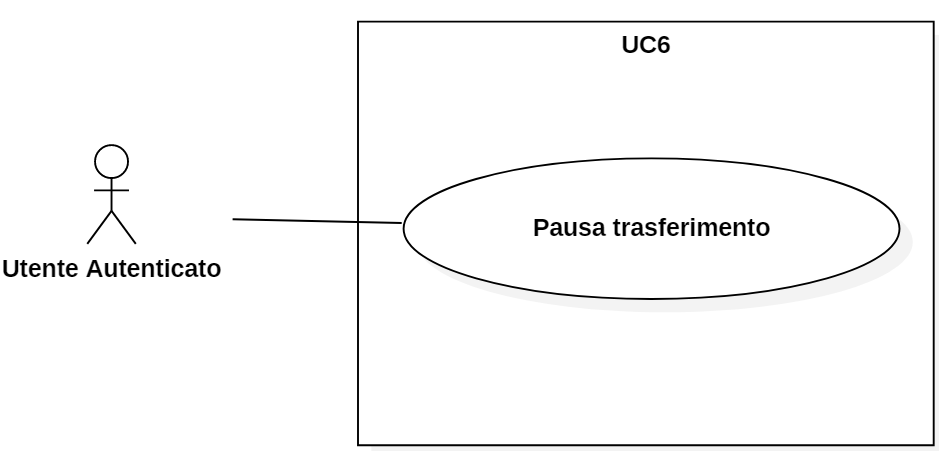
\includegraphics[scale = 0.7]{components/img/UC6.png}
    \caption{UC6 - Visualizza dettagli file}
\end{figure}
\begin{itemize}
\item \textbf{Attore Primario:} Utente autenticato;
\item \textbf{Precondizione:} L'utente ha selezionato la cartella root e sono presenti file al suo interno;
\item \textbf{Postcondizione:} L'utente ha informazioni riguardo al file;
\item \textbf{Scenario principale:} L'utente può visualizzare le informazioni riguardanti i file all'interno della cartella root selezionata.
\end{itemize}